% !TEX root = ../Planning.tex
\section{Project description}
\label{sec:project-description}

\subsection{The Ampersand project}
In November 2003, the Business Rules Manifesto\cite{business-rules} was written, with the main purpose of declaring independence for business rules in the world of requirements.
The manifesto supports the vision of business rules as equivalent to requirements.
This is considered a radical change on how people see the world of business architecture.

In December 2010, Stef Joosten, Lex Wedemeijer and Gerard Michels published the paper `Rule Based Design', presenting the Ampersand approach.
The approach puts the rules in the center, using them to define the business processes.
Ampersand is named after the \& symbol with the desire of realizing results for both business and IT, in an efficient and effective way.

In 2011, the Ampersand compiler was created as an open source project.
Since then, the compiler has been improved and applied in both business and academic contexts.
The Ampersand end-users write business rules in a specific language (ADL), and compile that specification into functional specification, documentation and working software prototypes.
\dict{ADL}{Ampersand Design Language}%
These rules are based on agreements between the different stakeholders.

The theory behind Ampersand has been throughly studied, and is based on mathe\-matical concepts, e.g. Relational algebra and Tarski's axioms.
Using this compiler, users write the requirements in ADL and generate all the system specification independent of the platform.
The main advantage is that the requirements consistency and traceability are always correct (and even provable), from the lowest level up to the front-end.
The requirements are presented to stakeholders in natural language, guaranteeing that any business expert who knows the context can validate the requirements.
\autoref{fig:generation} depicts the artifacts generated by the Ampersand compiler.
%
\begin{figure}[htb]
	\centering
	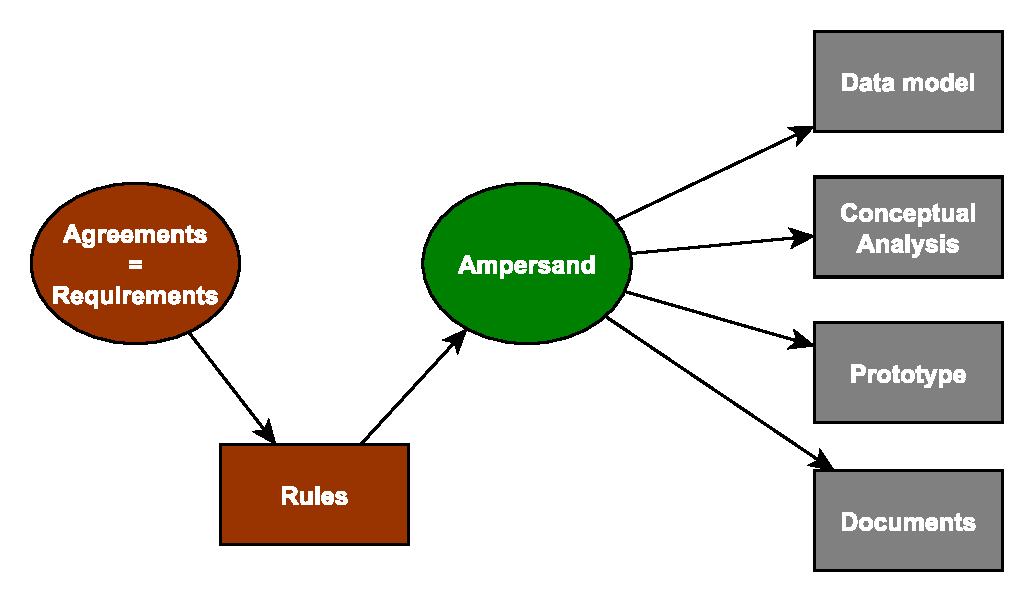
\includegraphics[width=0.7\textwidth]{Figures/Generation}
	\caption[Generated artifacts]{The Ampersand approach generates different artifacts based on the business rules}
	\label{fig:generation}
\end{figure}

\subsection{Project architecture and components}
\label{subsec:architecture}
The compiler developed for the Ampersand research project runs in several steps.
Thence the Ampersand compiler is also divided in several subcomponents:
\dict{P-structure}{The parse-tree generated by the Ampersand parser, used as input for the type checker.}%
\dict{A-structure}{The ADL code generated by the Ampersand type checker, used as input for the calculator component.}%
\dict{ADL-structure}{See A-structure.}%
\dict{F-structure}{The functional structure generated by the Ampersand calculator, used as input for the different output modules.}%
\begin{description}
	\item[Parser:] This component receives the ADL code as input, and parses that code into a parse-tree (also known as P-structure).
	\item[Type checker:] The Ampersand type checker receives the P-structure as input and converts it into a relational algebra format, suitable for manipulation (also known as A-structure or ADL-structure).
		 The semantics of ampersand are expressed in terms of the A-structure.
	\item[Calc:] The Calc component receives the A-structure as input, and manipulates it according to the research rules, generating the functional structure (also known as F-structure).
		The F-structure contains all design artifacts needed to write a specification and generate the output.
	\item[Output components:] All design artifacts present in the F-structure are ready to be rendered.
		Several components use this data structure to generate the wished output.
		The output components currently implemented (and their output formats) are the following: 
		\begin{itemize}
			\item Atlas (HTML interface);
			\item Revert (Haskell source);
			\item Query (prototype generation);
			\item Documentation Generator (Pandoc structure).
		\end{itemize}
\end{description}
%
The complete architecture is depicted in \autoref{fig:architecture}.
The part of this architecture relevant for this project is depicted in \autoref{fig:data-flow}.
%
\begin{figure}[htb]
	\centering
	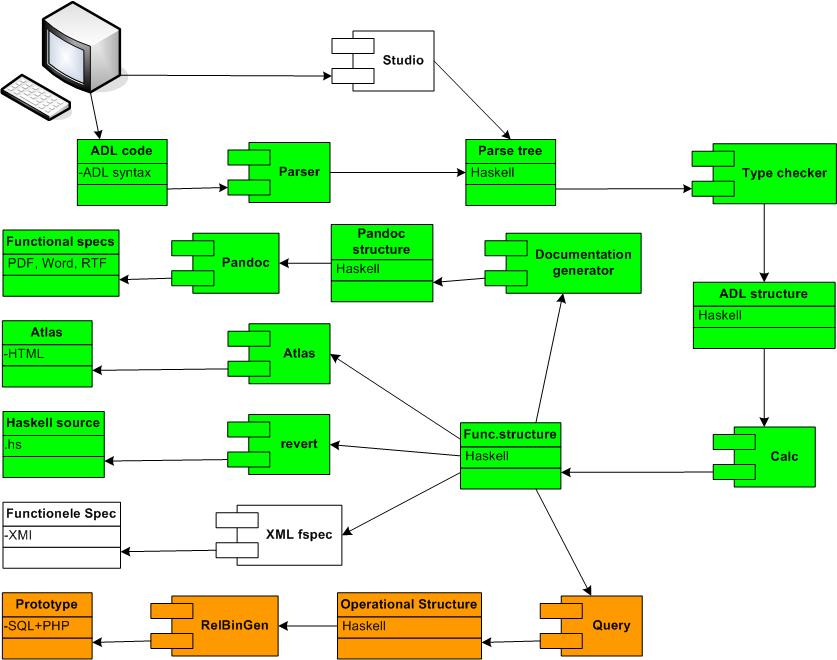
\includegraphics[width=\textwidth]{Figures/ADL_systeemarchitectuur}
	\caption[Architecture of the project]{Architecture of the project, showing where the parser fits in the Ampersand system}
	\label{fig:architecture}
	\small
	The components in green background are part of the Ampersand compiler.
	Components in orange are part of the Ampersand Prototype compiler.
	Finally, components in white background are future components, not yet implemented.
\end{figure}
%
\begin{figure}[htb]
	\centering
	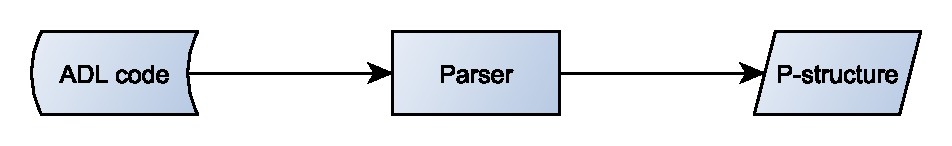
\includegraphics[width=0.5\textwidth]{Figures/Architecture}
	\caption{Relevant data flow for the Ampersand parsing component}
	\label{fig:data-flow}
\end{figure}

\subsection{Current situation}
The end-to-end process of the ampersand project, from compiling towards the generated artifacts is correct, however there is a major improvement topic identified in the first step, the parsing of the input scripts.

One of the main complaints from users is the quality of the errors generated by the Ampersand parser making it though for the end users to correct faulty ADL statements.
Since the beginning of the project, the parser subcomponent never received special attention, and it has not been analyzed for improvements.

In order to generate better, useful and to the point error messages, it is assumed that a complete refactoring of the parser will be necessary.
The main challenge is to choose the correct kind of architecture and libraries in order to generate the most user-friendly messages possible.

Besides the main project task of improving the parser's feedback, a list of user wishes has accumulated over the years.
The main customer and other users would appreciate if as many wishes as possible could be fulfilled.

\subsection{Goals of the project}
\label{subsec:project-goals}
The main objective for the graduation project is to implement useful feedback in the Ampersand parser.
In order to achieve this goal, the following research \& analysis activities will take place:
\begin{itemize}
	\item Analysis of user-friendly messages in compilers;
	\item Comparison of different Haskell parsing libraries (also for pretty-printing);
\end{itemize}
%
Additionally, the following activities may also take place:
\begin{itemize}
	\item Researching tools and techniques in Haskell for improving the software quality (e.g. testing and error messages);
	\item Analysis of the current development environment in relation with software engineering principles such as continuous delivery/integration;
	\item Recommending improvements for the overall software quality;
\end{itemize}
%
In case the new parser is successfully implemented and accepted, while the project members still have time budget available, the list of open user wishes issues can be addressed.
Some of these wishes are substantial, so that most of them cannot be fulfilled during the graduation project.
The current list of open issues has been provided\cite{open-issues}, although it must be clear that the issues are strictly seen as lower priority.
See also \autoref{sec:requirements} for the list of high-level requirements.

\subsection{Project environment}
The Ampersand project is used in the following environments, for different users:
\begin{description}
	\item[Research:] The Ampersand project is part of a research domain on the use of business rules for software design;
	\item[Academic:] Ampersand is used as main tool in the course `Ontwerpen met bedrijfsregels' (code T18321) from the Open Universiteit Nederland;
	\item[Business:] The compiler is used in business environments to design and develop real world business software.
\end{description}

\subsection{Critical success factors}
\label{subsec:success-factors}
The following factors are critical for the project's successful completion.
Each critical success factor is covered by one or more measures outlined in this project plan:
\begin{description}
	\item[Maintainability:] the code shall at least be as maintainable as the current Ampersand code.
		It is known however that maintainability is hard to measure (see also \autoref{sec:risk-management}).
	\item[Production code:] the implemented functionalities shall be integrated into the master branch for production use;
	\item[Users context:] in order to provide useful feedback, the user context wherein the Ampersand compiler is used needs to be well understood, and the improvements must have extra user value. 
		Just like maintainability, useful feedback is a hard to measure topic, this risk is listed in \autoref{sec:risk-management} and will be addressed in phase 3C (investigation context).
	\item[Communication:] Independent on how good the project results are, if the solution is put into production without proper communication and documentation leading to confused and demotivated users, the project will be perceived as a failure. 
	Although the project aims to add the feedback in the ampersand parser as transparent as possible, the final customer and user perception remains a critical success factor of this project;
\end{description}
%
The syntax of the Ampersand grammar is written in the the EBNF notation.
Any changes to the syntax must be documented according with this notation.
The notation can also be added as comment in the source code, in order to make clear that all the grammar is implemented completely and correctly.

\subsection{Objectives and commitments}
Besides the project goals described in \autoref{subsec:project-goals} and the customer goals described in \autoref{subsec:success-factors}, the project members declare herewith to have the following objectives and commitments fulfilled by the end of this graduation project:
\begin{description}
	\item[Customer:] The primary objective is to deliver a well-working and maintainable piece of software that will help the customer.
	\item[Users:] Another important goal is to make the software more user friendly, and so improve the usability.
	\item[Knowledge:] Building up knowledge is the main reason why one starts a bachelor study.
		As such it is important do learn more about functional programming, Haskell, compilers, business rules and research in general.
	\item[University:] Hopefully the final thesis will be of use for the university and other students.
	\item[Graduation:] As this is a graduation project, it is natural to have the graduation as an important objective.
\end{description}
